\let\negmedspace\undefined
\let\negthickspace\undefined
\documentclass[journal]{IEEEtran}
\usepackage[a5paper, margin=10mm, onecolumn]{geometry}
%\usepackage{lmodern} % Ensure lmodern is loaded for pdflatex
\usepackage{tfrupee} % Include tfrupee package

\setlength{\headheight}{1cm} % Set the height of the header box
\setlength{\headsep}{0mm}     % Set the distance between the header box and the top of the text

\usepackage{gvv-book}
\usepackage{gvv}
\usepackage{cite}
\usepackage{amsmath,amssymb,amsfonts,amsthm}
\usepackage{algorithmic}
\usepackage{graphicx}
\usepackage{textcomp}
\usepackage{xcolor}
\usepackage{txfonts}
\usepackage{listings}
\usepackage{enumitem}
\usepackage{mathtools}
\usepackage{gensymb}
\usepackage{comment}
\usepackage[breaklinks=true]{hyperref}
\usepackage{tkz-euclide} 
\usepackage{listings}
% \usepackage{gvv}                                        
\def\inputGnumericTable{}                                 
\usepackage[latin1]{inputenc}                                
\usepackage{color}                                            
\usepackage{array}                                            
\usepackage{longtable}                                       
\usepackage{calc}                                             
\usepackage{multirow}                                         
\usepackage{hhline}                                           
\usepackage{ifthen}                                           
\usepackage{lscape}
\usepackage{circuitikz}


\renewcommand{\thefigure}{\theenumi}
\renewcommand{\thetable}{\theenumi}
\setlength{\intextsep}{10pt} % Space between text and floats


\numberwithin{equation}{enumi}
\numberwithin{figure}{enumi}
\renewcommand{\thetable}{\theenumi}


% Marks the beginning of the document
\begin{document}
\bibliographystyle{IEEEtran}
\vspace{3cm}

\title{GATE CS 2012}
\author{EE25BTECH11011 - Banavathu Navya}
\maketitle

\begin{center}
 \textbf{Q.1 - Q.20 Carry One Mark Each.}
\end{center}
\begin{enumerate}
\item Which of the following problems are decidable?
\begin{enumerate}
    \item Does a given program ever produce an output?
    \item If L is context-free language, then, is L also context-free?
    \item If L is regular language, then, is L also regular?
    \item If L is recursive language, then, is L also recursiv
\end{enumerate}
\begin{enumerate}
\begin{multicols}{4}
    \item $1$,$2$,$3$,$4$
    \item $1$,$2$
    \item $2$,$3$,$4$
    \item $3$,$4$
\end{multicols}
\end{enumerate}

\item Given the language L-{ab, aa, baa}, which of the following strings are in L*? 
\begin{enumerate}
   \item abaabaaabaa
   \item aaaabaaaa
   \item baaaaabaaaab
   \item baaaa
\end{enumerate}
\begin{enumerate}
\begin{multicols}{4}
   \item $1$,$2$ and $3$
   \item $2$,$3$ and $4$
   \item $1$,$2$ and $4$
   \item $1$,$3$ and $4$
\end{multicols}
\end{enumerate}

\item In the IPv4 addressing format, the number of networks allowed under Class C addresses is
\begin{enumerate}
\begin{multicols}{4}
    \item $2^{14}$
    \item $2^{7}$
    \item $2^{21}$
    \item $2^{24}$
\end{multicols}
\end{enumerate}

\item Which of the following transport layer protocols is used to support electronic mail?
\begin{enumerate}
\begin{multicols}{4}
    \item SMTP
    \item IP
    \item TCP 
    \item UDP
\end{multicols}
\end{enumerate}

\item Consider a random variable X that takes values $+ 1$and $-1$ with probability $0.5$ each. The values of the cumulative distribution function F(x) at x = $-1$ and $+1$ are 
\begin{enumerate}
\begin{multicols}{2}
   \item $0$ and $0,5$
   \item $0$ and $1$
   \item $0.5$ and $1$
   \item $0,25$ and $0.75$
\end{multicols}
\end{enumerate}

\item Register renaming is done is pipelined processors
\begin{enumerate}
   \item as an alternative to register allocation at compile time
   \item for efficient access to function parameters and local variables
   \item to handle certain kinds of hazards
   \item as part of address translation 
\end{enumerate}

\item The amount of ROM needed to implement a 4 bit multiplier is
\begin{enumerate}
\begin{multicols}{4}
    \item $64$ bits
    \item $128$ bits
    \item $1$ Kbits
    \item $2$ Kbits
\end{multicols}
\end{enumerate}

\item Let $W(n)$ and $A(n)$ denote respectively, the worst case and average case running time of an algorithm executed on an input of size $n$.  
Which of the following is \textbf{ALWAYS TRUE}?
\begin{enumerate}
\begin{multicols}{2}
    \item $A(n) = \Omega(W(n))$ \quad
    \item $A(n) = \Theta(W(n))$ \quad 
    \item $A(n) = O(W(n))$ \quad 
    \item $A(n) = o(W(n))$ \quad
\end{multicols}
\end{enumerate}

\item Let G be a simple undirected planar graph on 10 vertices with $15$ edges. If G is a connected graph, then the number of bounded faces in any embedding of G on the plane is equal to 
\begin{enumerate}
\begin{multicols}{4}
    \item $3$
    \item $4$
    \item $5$
    \item $6$
\end{multicols}
\end{enumerate}

\item The recurrence relation capturing the optimal execution time of the Towers of Hanoi problem
with n discs is
\begin{enumerate}
\begin{multicols}{2}
   \item  T(n)=$2$T(n-$2$)+$2$
   \item  T(n)=$2$T(n-$1$)+n
   \item  T(n)=$2$T(n/$2$)+$1$
   \item  T(n)=$2$T(n-$1$)+$1$
\end{multicols}
\end{enumerate}

\item Which of the following statements are \textbf{TRUE}, about an SQL query?

\begin{enumerate}
    \item[P:] An SQL query can contain a \texttt{HAVING} clause even if it does not have a \texttt{GROUP BY} clause.
    \item[Q:] An SQL query can contain a \texttt{HAVING} clause only if it has a \texttt{GROUP BY} clause.
    \item[R:] All attributes used in the \texttt{GROUP BY} clause must appear in the \texttt{SELECT} clause.
    \item[S:] Not all attributes used in the \texttt{GROUP BY} clause need to appear in the \texttt{SELECT} clause.
\end{enumerate}

\begin{enumerate}
\begin{multicols}{2}
    \item P and R
    \item P and S
    \item Q and R
    \item Q and S
\end{multicols}
\end{enumerate}

\item Given the basic ER and relational models, which of the following is INCORRECT? 
\begin{enumerate}
    \item An attribute of an entity can have more than one value
    \item An attribute of an entity can be composite
    \item In a row of a relational table, an attribute can have more than one value
    \item In a row of a relational table, an attribute can have exactly one value or a NULL value 
\end{enumerate}

\item What is the complement of the language accepted by the NFA shown below?  
Assume $\Sigma = \{a\}$ and $\varepsilon$ is the empty string.
\begin{figure}[H]
    \centering
    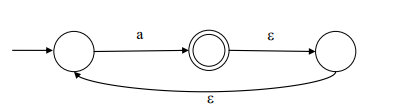
\includegraphics[width=0.5\columnwidth]{figs/New folder (2)/fig1.png}
    \caption{}
    \label{fig:3}
   \end{figure}
\begin{enumerate}
\begin{multicols}{4}
    \item $\varnothing$
    \item $\{\varepsilon\}$
    \item $a^{*}$
    \item $\{a, \varepsilon\}$
\end{multicols}
\end{enumerate}

\item What is the correct translation of the following statement into mathematical logic?  
\textit{``Some real numbers are rational''}
\begin{enumerate}
\begin{multicols}{2}
    \item $\exists x \; ( \text{real}(x) \lor \text{rational}(x))$
    \item $\forall x \; (\text{real}(x) \rightarrow \text{rational}(x))$
    \item $\exists x \; (\text{real}(x) \land \text{rational}(x))$
    \item $\exists x \; (\text{rational}(x) \rightarrow \text{real}(x))$
\end{multicols}
\end{enumerate}

\item Let $A$ be the $2 \times 2$ matrix with elements  
$a_{11} = a_{12} = a_{21} = +1$ and $a_{22} = -1$.  
Then the eigenvalues of the matrix $A^{19}$ are
\begin{enumerate}
\begin{multicols}{2}
    \item $1024$ and $-1024$
    \item $1024 \sqrt{2}$ and $-1024 \sqrt{2}$
    \item $4 \sqrt{2}$ and $-4 \sqrt{2}$
    \item $512 \sqrt{2}$ and $-512 \sqrt{2}$
\end{multicols}
\end{enumerate}

\item The protocol data unit (PDU) for the application layer in the Internet stack is
\begin{enumerate}
\begin{multicols}{4}
    \item Segment
    \item Datagram
    \item Message
    \item Frame 
\end{multicols}
\end{enumerate}

\item Consider the function $f(x) = \sin(x)$ in the interval $x \in \left[\tfrac{\pi}{4}, \tfrac{7\pi}{4}\right]$. 
  The number and location(s) of the local minima of this function are  
\begin{enumerate}
\begin{multicols}{2}
    \item One, at $\tfrac{\pi}{2}$
    \item One, at $\tfrac{3\pi}{2}$
    \item Two, at $\tfrac{\pi}{2}$ and $\tfrac{3\pi}{2}$
    \item Two, at $\tfrac{\pi}{4}$ and $\tfrac{3\pi}{2}$
\end{multicols}
\end{enumerate}
  
\item A process executes the code
  \begin{verbatim}
  fork();
  fork();
  fork();
  \end{verbatim}
  The total number of child processes created is  
  \begin{enumerate}
  \begin{multicols}{4}
    \item $3$
    \item $4$
    \item $7$
    \item $8$
\end{multicols}
\end{enumerate}
  
\item The decimal value $0.5$ in IEEE single precision floating point representation has  
\begin{enumerate}
    \item fraction bits of $000\ldots000$ and exponent value of $0$
    \item fraction bits of $000\ldots000$ and exponent value of $-1$
    \item fraction bits of $100\ldots000$ and exponent value of $0$
    \item no exact representation
\end{enumerate}

\item The truth table  
  \[
  \begin{array}{|c|c|c|}
  \hline
  X & Y & f(X,Y) \\
  \hline
  0 & 0 & 0 \\
  0 & 1 & 0 \\
  1 & 0 & 1 \\
  1 & 1 & 1 \\
  \hline
  \end{array}
  \]
  represents the Boolean function
\begin{enumerate}
\begin{multicols}{4}
    \item $X$
    \item $X+Y$
    \item $X \oplus Y$
    \item $Y$
\end{multicols}
\end{enumerate}
  
\item The worst case running time to search for an element in a balanced binary search tree with $n^{2}$ elements is
\begin{enumerate}
\begin{multicols}{4}
    \item $\Theta(n \log n)$
    \item $\Theta(n^{2^n})$
    \item $\Theta(n)$
    \item $\Theta(\log n)$
\end{multicols}
\end{enumerate}  
  
\item Assuming $P \ne NP$, which of the following is TRUE?
  \begin{enumerate}
  \begin{multicols}{2}
    \item NP-complete $=$ NP
    \item NP-complete $\cap$ P $= \varnothing$
    \item NP-hard $=$ NP
    \item P $=$ NP-complete
\end{multicols}
\end{enumerate}

\item What will be the output of the following C program segment?

\begin{lstlisting}[language=C]
char inChar = 'A';
switch (inChar) {
    case 'A': printf("Choice A\n");
    case 'B': 
    case 'C': printf("Choice B");
    case 'D': 
    case 'E': 
    default : printf("No Choice");
}
\end{lstlisting}

\begin{enumerate}
    \item No choice
    \item Choice A
    \item Choice A 
          Choice B No choice
    \item Program gives no output as it is erroneous
\end{enumerate}

\item Which of the following is TRUE? 
\begin{enumerate}
    \item  Every relation is $3$NF is also in BCNF
    \item A relation R is in $3$NF if every non-prime attribute of R is fully functionally dependent on
every key of R
    \item Every relation in BCNF is also in $3$NF
    \item No relation can be in both BCNF and $3$NF 
\end{enumerate}

\item Consider the following logical inferences:

$I_1 : \quad \text{If it rains then the cricket match will not be played.} $
$\text{The cricket match was played.}$
$\text{Inference: There was no rain.}$

$I_2 : \quad \text{If it rains then the cricket match will not be played.} $
$\text{It did not rain.}$
$\text{Inference: The cricket match was played.}$

Which of the following is \textbf{TRUE}?
\begin{enumerate}
    \item Both $I_1$ and $I_2$ are correct inferences
    \item $I_1$ is correct but $I_2$ is not a correct inference
    \item $I_1$ is not correct but $I_2$ is a correct inference
    \item Both $I_1$ and $I_2$ are not correct inferences
\end{enumerate}


\begin{center}
 \textbf{Q.26 - Q.55 Carry Two Marks Each.}
\end{center}

\item Which of the following graphs is isomorphic to
\begin{figure}[H]
    \centering
    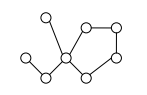
\includegraphics[width=0.3\columnwidth]{figs/New folder (2)/fig2.png}
    \caption{isomorphic}
    \label{fig:2}
   \end{figure}
\begin{enumerate}
\begin{multicols}{2}
    \item 
    \begin{figure}[H]
    \centering
    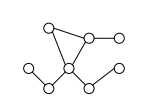
\includegraphics[width=0.5\columnwidth]{figs/New folder (2)/fig3.png}
    \caption{A}
    \label{fig:3}
   \end{figure}
   \item
   \begin{figure}[H]
    \centering
    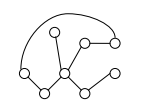
\includegraphics[width=0.5\columnwidth]{figs/New folder (2)/fig4.png}
    \caption{B}
    \label{fig:4}
   \end{figure}
   \item 
   \begin{figure}[H]
    \centering
    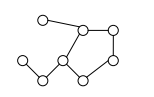
\includegraphics[width=0.5\columnwidth]{figs/New folder (2)/fig5.png}
    \caption{C}
    \label{fig:5}
   \end{figure}
   \item 
   \begin{figure}[H]
    \centering
    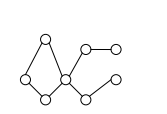
\includegraphics[width=0.5\columnwidth]{figs/New folder (2)/fig6.png}
    \caption{D}
    \label{fig:6}
   \end{figure}
\end{multicols}
\end{enumerate}


\item Consider the following transactions with data items $P$ and $Q$ initialized to zero:

$
T_1 : \quad 
\begin{array}{l}
\text{read}(P); \\
\text{read}(Q); \\
\text{if } P = 0 \text{ then } Q := Q + 1; \\
\text{write}(Q);
\end{array}
$

$
T_2 : \quad 
\begin{array}{l}
\text{read}(Q); \\
\text{read}(P); \\
\text{if } Q = 0 \text{ then } P := P + 1; \\
\text{write}(P);
\end{array}
$

Any non-serial interleaving of $T_1$ and $T_2$ for concurrent execution leads to:

\begin{enumerate}
    \item a serializable schedule
    \item a schedule that is not conflict serializable
    \item a conflict serializable schedule
    \item a schedule for which a precedence graph cannot be drawn
\end{enumerate}

\item The bisection method is applied to compute a zero of the function
$f(x) = x^4 - x^3 - x^2 - 4$
in the interval $[1,9]$.  
The method converges to a solution after $\_\_\_$ iterations.
\begin{enumerate}
\begin{multicols}{4}
    \item $1$
    \item $3$
    \item $5$
    \item $7$
\end{multicols}
\end{enumerate}

\item Let $G$ be a weighted graph with edge weights greater than one, and let $G'$ be the graph constructed by squaring the weights of edges in $G$.  
Let $T$ and $T'$ be the minimum spanning trees of $G$ and $G'$, respectively, with total weights $t$ and $t'$.  
Which of the following statements is \textbf{TRUE}?

\begin{enumerate}
    \item $T' = T$ with total weight $t' = t^2$
    \item $T' = T$ with total weight $t' < t^2$
    \item $T' \neq T$ but total weight $t' = t^2$
    \item None of the above
\end{enumerate}

\item What is the minimal form of the Karnaugh map shown below?  
Assume that $X$ denotes a don't care term.
\begin{figure}[H]
    \centering
    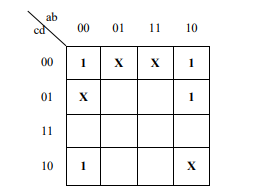
\includegraphics[width=0.5\columnwidth]{figs/New folder (2)/fig7.png}
    \caption{Karnaugh map}
    \label{fig:7}
   \end{figure}
\begin{enumerate}
\begin{multicols}{4}
    \item $\bar{b}\bar{d}$
    \item $\bar{b}\bar{d} + \bar{b}\bar{c}$
    \item $\bar{b}\bar{d} + a\bar{b}\bar{c}d$
    \item $\bar{b}\bar{d} + \bar{b}\bar{c} + \bar{c}\bar{d}$
\end{multicols}
\end{enumerate}

\item Consider the 3 processes, $P1, P2, P3$ shown in the table.
$
\begin{array}{|c|c|c|}
\hline
\text{Process} & \text{Arrival Time} & \text{Time Units Required} \\
\hline
P1 & 1 & 5 \\
P2 & 1 & 7 \\
P3 & 3 & 4 \\
\hline
\end{array}
$

The completion order of the $3$ processes under the policies FCFS and RR$2$ (round robin scheduling with CPU quantum of $2$ time units) are:

\begin{enumerate}
\begin{multicols}{2}
    \item FCFS: P$1$, P$2$, P$3$ \quad RR$2$: P$1$, P$2$, P$3$
    \item FCFS: P$1$, P$3$, P$2$ \quad RR$2$: P$1$, P$3$, P$2$
    \item FCFS: P$1$, P$2$, P$3$ \quad RR$2$: P$1$, P$3$, P$2$
    \item FCFS: P$1$, P$3$, P$2$ \quad RR$2$: P$1$, P$2$, P$3$
\end{multicols}
\end{enumerate}

\item \texttt{Fetch\_And\_Add(X,i)} is an atomic Read-Modify-Write instruction that reads the value of memory location $X$, increments it by the value $i$, and returns the old value of $X$.  
It is used in the pseudocode shown below to implement a busy-wait lock.  
$L$ is an unsigned integer shared variable initialized to $0$.  
The value $0$ corresponds to lock being available, while any non-zero value corresponds to lock not being available.

\begin{verbatim}
AcquireLock(L) {
    while (Fetch_And_Add(L,1))
        L = 1;
}

ReleaseLock(L) {
    L = 0;
}
\end{verbatim}

This implementation

\begin{enumerate}
    \item fails as $L$ can overflow
    \item fails as $L$ can take on a non-zero value when the lock is actually available
    \item works correctly but may starve some processes
    \item works correctly without starvation
\end{enumerate}

\item Suppose a fair six-sided die is rolled once.  
If the value on the die is $1$, $2$, or $3$, the die is rolled a second time.  
What is the probability that the sum total of values that turn up is at least $6$?

\begin{enumerate}
\begin{multicols}{4}   
    \item $\tfrac{10}{21}$
    \item $\tfrac{5}{12}$
    \item $\tfrac{2}{3}$
    \item $\tfrac{1}{6}$
\end{multicols}
\end{enumerate}
 
\item An Internet Service Provider (ISP) has the following chunk of CIDR-based IP addresses available with it:  
$245.248.128.0/20$ 
The ISP wants to give half of this chunk of addresses to Organization A, and a quarter to Organization B, while retaining the remaining with itself.  
Which of the following is a valid allocation of addresses to A and B?

\begin{enumerate}
    \item $245.248.136.0/21$ and $245.248.128.0/22$
    \item $245.248.128.0/21$ and $245.248.128.0/22$
    \item $245.248.132.0/22$ and $245.248.132.0/21$
    \item $245.248.136.0/24$ and $4245.248.132.0/21$
\end{enumerate}

\item Suppose a circular queue of capacity $(n-1)$ elements is implemented with an array of $n$ elements.  
Assume that the insertion and deletion operations are carried out using \texttt{REAR} and \texttt{FRONT} as array index variables, respectively.  
Initially, \texttt{REAR = FRONT = 0}.  
The conditions to detect \emph{queue full} and \emph{queue empty} are:

\begin{enumerate}
    \item \textbf{full:} $(REAR+1) \bmod n = FRONT$ 
          \textbf{empty:} $REAR = FRONT$
    \item \textbf{full:} $(REAR+1) \bmod n = FRONT$ 
          \textbf{empty:} $(FRONT+1) \bmod n = REAR$
    \item \textbf{full:} $REAR = FRONT$ 
          \textbf{empty:} $(REAR+1) \bmod n = FRONT$
    \item \textbf{full:} $(FRONT+1) \bmod n = REAR$ 
          \textbf{empty:} $REAR = FRONT$
\end{enumerate}

\item Consider the program given below, in a block-structured pseudo-language with lexical scoping and nesting of procedures permitted.

\begin{lstlisting}[language=Pascal]
Program main;
Var ...
   Procedure A1;
      Var ...
      Call A2;
   End A1;

   Procedure A2;
      Var ...
      Procedure A21;
         Var ...
         Call A1;
      End A21;

      Call A21;
   End A2;

   Call A1;
End main.
\end{lstlisting}

Consider the calling chain:  
$
\text{Main} \;\rightarrow\; A1 \;\rightarrow\; A2 \;\rightarrow\; A21 \;\rightarrow\; A1
$

The correct set of activation records along with their access links is given by:
\begin{enumerate}
\begin{multicols}{2}
    \item 
    \begin{figure}[H]
    \centering
    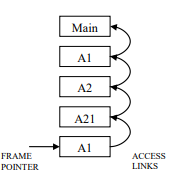
\includegraphics[width=0.5\columnwidth]{figs/New folder (2)/fig8.png}
    \caption{A}
    \label{fig:8}
   \end{figure}
   \item \begin{figure}[H]
    \centering
    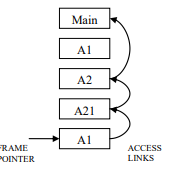
\includegraphics[width=0.5\columnwidth]{figs/New folder (2)/fig9.png}
    \caption{B}
    \label{fig:9}
   \end{figure}
   \item \begin{figure}[H]
    \centering
    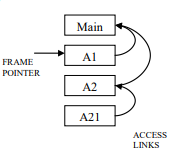
\includegraphics[width=0.5\columnwidth]{figs/New folder (2)/fig10.png}
    \caption{C}
    \label{fig:10}
   \end{figure}
   \item \begin{figure}[H]
    \centering
    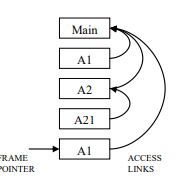
\includegraphics[width=0.5\columnwidth]{figs/New folder (2)/fig11.png}
    \caption{D}
    \label{fig:11}
   \end{figure}
\end{multicols}
\end{enumerate}

\item How many onto (or surjective) functions are there from an $n$-element ($n \geq 2$) set to a 2-element set?

\begin{enumerate}
\begin{multicols}{4}
    \item $2^n$
    \item $2^n - 1$
    \item $2^n - 2$
    \item $2(2^{n-1} - 1)$
\end{multicols}
\end{enumerate}

\item Let $G$ be a complete undirected graph on 6 vertices. If vertices of $G$ are labeled, then the number of distinct cycles of length 4 in $G$ is equal to

\begin{enumerate}
\begin{multicols}{4}
    \item $15$
    \item $30$
    \item $90$
    \item $360$
 \end{multicols}
\end{enumerate}

\item A list of $n$ strings, each of length $n$, is sorted into lexicographic order using the merge-sort algorithm. The worst-case running time of this computation is

\begin{enumerate}
\begin{multicols}{4}
    \item $O(n \log n)$
    \item $O(n^2 \log n)$
    \item $O(n^2 + \log n)$
    \item $O(n^2)$
\end{multicols}
\end{enumerate}

\item Consider the directed graph shown in the figure below.  
There are multiple shortest paths between vertices $S$ and $T$. Which one will be reported by Dijkstra's shortest path algorithm?
\begin{figure}[H]
    \centering
    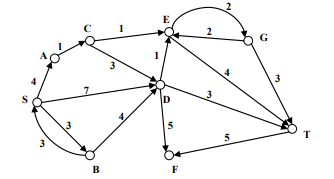
\includegraphics[width=0.5\columnwidth]{figs/New folder (2)/fig12.png}
    \caption{Graph}
    \label{fig:12}
   \end{figure}
\begin{enumerate}
\begin{multicols}{4}
    \item SDT
    \item SBDT
    \item SACDT
    \item SACET
\end{multicols}
\end{enumerate}

\item A file system with $300$ GByte disk uses a file descriptor with $8$ direct block addresses, $1$ indirect block address and $1$ doubly indirect block address. The size of each disk block is $128$ Bytes and the size of each disk block address is $8$ Bytes. The maximum possible file size in this file system is

\begin{enumerate}
    \item $3$ KBytes
    \item $35$ KBytes
    \item $280$ KBytes
    \item Dependent on the size of the disk
\end{enumerate}

\item Consider the virtual page reference string:  
$
1, 2, 3, 2, 4, 1, 3, 2, 4, 1
$
on a demand paged virtual memory system running on a computer system that has main memory size of 3 page frames which are initially empty.  

Let LRU, FIFO, and OPTIMAL denote the number of page faults under the corresponding page replacement policy. Then

\begin{enumerate}
    \item OPTIMAL $<$ LRU $<$ FIFO
    \item OPTIMAL $<$ FIFO $<$ LRU
    \item OPTIMAL = LRU
    \item OPTIMAL = FIFO
\end{enumerate}

\item Suppose $R_1(A, B)$ and $R_2(C, D)$ are two relation schemas.  
Let $r_1$ and $r_2$ be the corresponding relation instances.  
$B$ is a foreign key that refers to $C$ in $R_2$.  

If data in $r_1$ and $r_2$ satisfy referential integrity constraints, which of the following is \textbf{ALWAYS TRUE}?

\begin{enumerate}
    \item $\Pi_B(r_1) - \Pi_C(r_2) = \emptyset$
    \item $\Pi_B(r_1) - \Pi_C(r_2) \neq \emptyset$
    \item $\Pi_C(r_2) - \Pi_B(r_1) = \emptyset$
    \item $\Pi_C(r_2) - \Pi_B(r_1) \neq \emptyset$
\end{enumerate}

\item Consider a source computer (S) transmitting a file of size $10^6$ bits to a destination computer (D) over a network of two routers ($R_1$ and $R_2$) and three links ($L_1, L_2,$ and $L_3$).  

$L_1$ connects $S$ to $R_1$, $L_2$ connects $R_1$ to $R_2$, and $L_3$ connects $R_2$ to $D$.  

Let each link be of length 100 km and signals travel over each link at a speed of $10^8$ meters per second. Assume that the link bandwidth on each link is 1 Mbps. Let the file be broken down into 1000 packets each of size 1000 bits.  

Find the total sum of transmission and propagation delays in transmitting the file from $S$ to $D$.

\begin{enumerate}
\begin{multicols}{4}
    \item $1005$ ms
    \item $1010$ ms
    \item $3000$ ms
    \item $3003$ ms
\end{multicols}
\end{enumerate}

\item Consider an instance of TCP's Additive Increase Multiplicative Decrease (AIMD) algorithm where the window size at the start of the slow start phase is 2 MSS and the threshold at the start of the first transmission is 8 MSS. Assume that a timeout occurs during the fifth transmission.  

Find the congestion window size at the end of the tenth transmission.

\begin{enumerate}
\begin{multicols}{4}
    \item $8$ MSS
    \item $14$ MSS
    \item $7$ MSS
    \item $12$ MSS
\end{multicols}
\end{enumerate}

\item Consider the set of strings on $\{0,1\}$ in which \emph{every substring of 3 symbols has at most two zeros}.  
For example, $001110$ and $01001$ are in the language, but $100010$ is not.  
All strings of length less than 3 are also in the language.  
A partially completed DFA that accepts this language is shown below.
\begin{figure}[H]
    \centering
    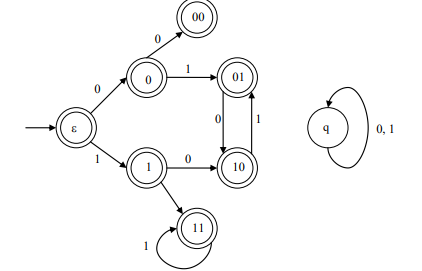
\includegraphics[width=0.5\columnwidth]{figs/New folder (2)/fig13.png}
    \caption{set of strings}
    \label{fig:13}
   \end{figure}

The missing arcs in the DFA are to be determined.
\begin{center}
\begin{tabular}{cc}
(A) 
\begin{tabular}{|c|c|c|c|c|c|}
\hline
   & 00 & 01 & 10 & 11 & q \\ \hline
00 & 1  & 0  &    &    &   \\ \hline
01 &    &    &    & 1  &   \\ \hline
10 & 0  &    &    &    &   \\ \hline
11 &    &    & 0  &    &   \\ \hline
\end{tabular}

(B) 
\begin{tabular}{|c|c|c|c|c|c|}
\hline
   & 00 & 01 & 10 & 11 & q \\ \hline
00 &    & 0  &    &    & 1 \\ \hline
01 &    & 1  &    &    &   \\ \hline
10 &    &    &    & 0  &   \\ \hline
11 &    & 0  &    &    &   \\ \hline
\end{tabular}
\\[1cm]
(C) 
\begin{tabular}{|c|c|c|c|c|c|}
\hline
   & 00 & 01 & 10 & 11 & q \\ \hline
00 &    & 1  &    &    & 0 \\ \hline
01 &    & 1  &    &    &   \\ \hline
10 &    &    & 0  &    &   \\ \hline
11 &    & 0  &    &    &   \\ \hline
\end{tabular}

(D) 
\begin{tabular}{|c|c|c|c|c|c|}
\hline
   & 00 & 01 & 10 & 11 & q \\ \hline
00 &    & 1  &    &    & 0 \\ \hline
01 &    &    &    & 1  &   \\ \hline
10 & 0  &    &    &    &   \\ \hline
11 &    &    & 0  &    &   \\ \hline
\end{tabular}
\end{tabular}
\end{center}


\item The height of a tree is defined as the number of edges on the longest path in the tree.  
The function shown in the pseudocode below is invoked as \texttt{height(root)} to compute the height of a binary tree rooted at the tree pointer \texttt{root}.

\begin{lstlisting}[language=C, basicstyle=\ttfamily\small]
int height (treeptr n)
{
    if (n == NULL) return -1;
    if (n -> left == NULL)
        if (n -> right == NULL) return 0;
        else return B1;    // Box 1
    else {
        h1 = height(n -> left);
        if (n -> right == NULL) return (1 + h1);
        else { 
            h2 = height(n -> right);
            return B2;    // Box 2
        }
    }
}
\end{lstlisting}

\noindent
The appropriate expressions for the two boxes B1 and B2 are:
$
\begin{array}{ll}
\text{(A)} & \text{B1: } (1 + \text{height}(n \to \text{right})) \quad 
              \text{B2: } (1 + \max(h1, h2)) \\[6pt]
\text{(B)} & \text{B1: } \text{height}(n \to \text{right}) \quad 
              \text{B2: } (1 + \max(h1, h2)) \\[6pt]
\text{(C)} & \text{B1: } \text{height}(n \to \text{right}) \quad 
              \text{B2: } \max(h1, h2) \\[6pt]
\text{(D)} & \text{B1: } (1 + \text{height}(n \to \text{right})) \quad 
              \text{B2: } \max(h1, h2) \\
\end{array}
$


\textbf{Common Data Questions} \\
\textbf{Common Data for Questions 48 and 49:} \\[4pt]
Consider the following C code segment.

\begin{lstlisting}[language=C, basicstyle=\ttfamily\small]
int a, b, c = 0;
void prtFun(void);

main()
{
    static int a = 1;    /* Line 1 */
    prtFun();
    a += 1;
    prtFun();
    printf("\n %d %d", a, b);
}

void prtFun(void)
{
    static int a = 2;    /* Line 2 */
    int b = 1;
    a += ++b;
    printf("\n %d %d", a, b);
}
\end{lstlisting}

\item What output will be generated by the given code segment?

$
\begin{array}{c@{\hspace{2cm}}c@{\hspace{2cm}}c@{\hspace{2cm}}c}
\text{(A)} &
\begin{array}{cc}
3 & 1 \\ 4 & 1 \\ 4 & 2
\end{array}
&
\text{(B)} &
\begin{array}{cc}
4 & 2 \\ 6 & 1 \\ 6 & 1
\end{array}
\\[1cm]
\text{(C)} &
\begin{array}{cc}
4 & 2 \\ 6 & 2 \\ 2 & 0
\end{array}
&
\text{(D)} &
\begin{array}{cc}
3 & 1 \\ 5 & 2 \\ 5 & 2
\end{array}
\end{array}
$

\item What output will be generated by the given code segment if:  

Line 1 is replaced by \verb|auto int a = 1;|  
Line 2 is replaced by \verb|register int a = 2;|

$
\begin{array}{c@{\hspace{2cm}}c@{\hspace{2cm}}c@{\hspace{2cm}}c}
\text{(A)} &
\begin{array}{cc}
3 & 1 \\ 4 & 1 \\ 4 & 2
\end{array}
&
\text{(B)} &
\begin{array}{cc}
4 & 2 \\ 6 & 1 \\ 6 & 1
\end{array}
\\[1cm]
\text{(C)} &
\begin{array}{cc}
4 & 2 \\ 6 & 2 \\ 2 & 0
\end{array}
&
\text{(D)} &
\begin{array}{cc}
4 & 2 \\ 4 & 2 \\ 2 & 0
\end{array}
\end{array}
$

\textbf{Common Data for Questions 50 and 51:} \\[6pt]

Consider the following relations $A$, $B$ and $C$:

$
\begin{array}{|c|c|c|}
\hline
\textbf{Id} & \textbf{Name} & \textbf{Age} \\
\hline
12 & Arun   & 60 \\
15 & Shreya & 24 \\
99 & Rohit  & 11 \\
\hline
\end{array}
\quad
\begin{array}{|c|c|c|}
\hline
\textbf{Id} & \textbf{Name} & \textbf{Age} \\
\hline
15 & Shreya & 24 \\
25 & Hari   & 40 \\
98 & Rohit  & 20 \\
99 & Rohit  & 11 \\
\hline
\end{array}
\quad
\begin{array}{|c|c|c|}
\hline
\textbf{Id} & \textbf{Phone} & \textbf{Area} \\
\hline
10 & 2200 & 02 \\
99 & 2100 & 01 \\
\hline
\end{array}
$

\item How many tuples does the result of the following relational algebra expression contain? Assume that the schema of $A \cup B$ is the same as that of $A$.  

$
(A \cup B) \bowtie_{A.Id > 40 \,\vee\, C.Id < 15} C
$

\begin{enumerate}
\begin{multicols}{4}
   \item $7$ 
   \item $4$
   \item $5$
   \item $9$
\end{multicols}
\end{enumerate}


\item How many tuples does the result of the following SQL query contain?

\begin{verbatim}
SELECT A.Id
FROM A
WHERE A.Age > ALL (SELECT B.Age
                   FROM B
                   WHERE B.Name = 'Arun');
\end{verbatim}

\begin{enumerate}
\begin{multicols}{4}
   \item $4$ 
   \item $3$
   \item $0$
   \item $1$
\end{multicols}
\end{enumerate}

\section*{Linked Answer Questions}

\subsection*{Statement for Linked Answer Questions 52 and 53:}

For the grammar below, a partial LL(1) parsing table is also presented along with the grammar. Entries that need to be filled are indicated as E1, E2, and E3. $\epsilon$ is the empty string, \$ indicates end of input, and $|$ separates alternate right hand sides of productions.

$
\begin{aligned}
S &\to aAB \;|\; bAaB \;|\; \epsilon 
A &\to S 
B &\to S
\end{aligned}
$

$
\begin{array}{|c|c|c|c|}
\hline
 & a & b & \$ \\
\hline
S & E1 & E2 & S \to \epsilon \\
\hline
A & A \to S & A \to S & \text{error} \\
\hline
B & B \to S & B \to S & E3 \\
\hline
\end{array}
$

\item The FIRST and FOLLOW sets for the non-terminals A and B are:
\begin{enumerate}
\item $\quad FIRST(A) = \{a,b,\epsilon\} = FIRST(B), \quad FOLLOW(A) = \{a,b\}, \quad FOLLOW(B) = \{a,b,\$\}$

\item $ \quad FIRST(A) = \{a,b,\$\}, \quad FIRST(B) = \{a,b,\epsilon\}, \quad FOLLOW(A) = \{a,b\}, \quad FOLLOW(B) = \{\$\} $

\item $ \quad FIRST(A) = \{a,b,\epsilon\} = FIRST(B), \quad FOLLOW(A) = \{a,b\}, \quad FOLLOW(B) = \emptyset
$
\item $ \quad FIRST(A) = \{a,b\} = FIRST(B), \quad FOLLOW(A) = \{a,b\}, \quad FOLLOW(B) = \{a,b\}$
\end{enumerate}

\item The appropriate entries for E$1$, E$2$, and E$3$ are:
\begin{enumerate}
\item $\quad E1: S \to aAB,\; A \to S \quad
E2: S \to bAaB,\; B \to S \quad
E3: B \to S$
\item $\quad E1: S \to aAB,\; S \to \epsilon \quad
E2: S \to bAaB,\; S \to \epsilon \quad
E3: S \to \epsilon$
\item $\quad E1: S \to aAB,\; S \to \epsilon \quad
E2: S \to bAaB,\; S \to \epsilon \quad
E3: B \to S$
\item $\quad E1: A \to S,\; S \to \epsilon \quad
E2: B \to S,\; S \to \epsilon \quad
E3: B \to S$
\end{enumerate}


\subsection*{Statement for Linked Answer Questions 54 and 55:}

A computer has a $256$ KByte, $4$-way set associative, write back data cache with block size of $32$ Bytes. The processor sends $32$ bit addresses to the cache controller. Each cache tag directory entry contains, in addition to address tag, $2$ valid bits, $1$ modified bit and $1$ replacement bit.

\item The number of bits in the tag field of an address is:
\begin{enumerate}
\begin{multicols}{4}
   \item $11$ 
   \item $14$
   \item $16$
   \item $27$
\end{multicols}
\end{enumerate}

\item The size of the cache tag directory is:
\begin{enumerate}
\begin{multicols}{4}
   \item $160$ Kbits
   \item $14$ Kbits
   \item $16$ Kbits
   \item $27$ Kbits
\end{multicols}
\end{enumerate}

\item The cost function for a product in a firm is given by $5q^2$, where $q$ is the amount of production. The firm can sell the product at a market price of \rupee50 per unit. The number of units to be produced by the firm such that the profit is maximized is:
\begin{enumerate}
\begin{multicols}{4}
   \item $5$ 
   \item $10$
   \item $15$
   \item $25$
\end{multicols}
\end{enumerate}

\item Choose the most appropriate alternative from the options given below to complete the following sentence:  

\textbf{Despite several \_\_\_\_ the mission succeeded in its attempt to resolve the conflict.}
\begin{enumerate}
\begin{multicols}{4}
   \item attempts
   \item setbacks
   \item meetings
   \item delegations
\end{multicols}
\end{enumerate}

\item Which one of the following options is the closest in meaning to the word given below?  

\textbf{Mitigate}  
\begin{enumerate}
\begin{multicols}{4}
   \item Diminish 
   \item Divulge
   \item Dedicate
   \item Denote
\end{multicols}
\end{enumerate}

\item Choose the grammatically INCORRECT sentence:

\begin{enumerate}
\item They gave us the money back less the service charges of Three Hundred rupees.  
\item This country's expenditure is not less than that of Bangladesh.  
\item The committee initially asked for a funding of Fifty Lakh rupees, but later settled for a lesser sum.  
\item This country's expenditure on educational reforms is very less.  
\end{enumerate}

\item Choose the most appropriate alternative from the options given below to complete the following sentence:  

\textbf{Suresh dog is the one \_\_\_\_ was hurt in the stampede.}  
\begin{enumerate}
\begin{multicols}{4}
   \item that
   \item which
   \item who
   \item whom
\end{multicols}
\end{enumerate}

\section*{Q.61 -- Q.65 carry two marks each.}

\item Wanted Temporary, Part-time persons for the post of Field Interviewer to conduct personal interviews to collect and collate economic data. Requirements: High School-pass, must be available for Day, Evening and Saturday work. Transportation paid, expenses reimbursed.  

Which one of the following is the best inference from the above advertisement?  

\begin{enumerate}
   \item Gender-discriminatory 
   \item Xenophobic
   \item Not designed to make the post attractive
   \item Not gender-discriminatory
\end{enumerate}

\item A political party orders an arch for the entrance to the ground in which the annual convention is being held. The profile of the arch follows the equation 
$ y = 2x - 0.1x^2 $
where $y$ is the height of the arch in meters. The maximum possible height of the arch is:  
\begin{enumerate}
\begin{multicols}{4}
    \item $8$ meters
    \item $10$ meters
    \item $12$ meters
    \item $14$ meters
    \end{multicols}
\end{enumerate}

\item  An automobile plant contracted to buy shock absorbers from two suppliers $X$ and $Y$.  
$X$ supplies 60\% and $Y$ supplies 40\% of the shock absorbers.  
All shock absorbers are subjected to a quality test. The ones that pass the quality test are considered reliable.  
Of $X$'s shock absorbers, 96\% are reliable. Of $Y$'s shock absorbers, 72\% are reliable.  

The probability that a randomly chosen shock absorber, which is found to be reliable, is made by $Y$ is

\begin{enumerate}
\begin{multicols}{4}
\item $0.288$
\item $0.334$
\item $0.667$
\item $0.720$
\end{multicols}
\end{enumerate}

\item  Which of the following assertions are \textbf{CORRECT}?  

\begin{enumerate}
\item Adding $7$ to each entry in a list adds $7$ to the mean of the list  
\item Adding $7$ to each entry in a list adds $7$ to the standard deviation of the list  
\item Doubling each entry in a list doubles the mean of the list  
\item Doubling each entry in a list leaves the standard deviation of the list unchanged  
\end{enumerate}

\begin{enumerate}
\begin{multicols}{4}
\item P, Q
\item Q, R
\item P, R
\item R, S
\end{multicols}
\end{enumerate}

\item Given the sequence of terms, $AD, CG, FK, JP$, the next term is  

\begin{enumerate}
\begin{multicols}{4}
\item OV
\item OW
\item PV
\item PW
\end{multicols}
\end{enumerate}


\end{enumerate}
\end{document}

